\documentclass[11pt]{article}

\usepackage{graphicx,color,setspace,amssymb,amsmath,amsthm,caption,subcaption,minted}
\usepackage[margin=1in, paperwidth=8.5in, paperheight=11in]{geometry}


% symbols
\def\deg{\ensuremath{^{\circ}}}
\def\ang{\AA{}}

% markup macros
\newcommand{\software}[1]{{\sc #1}}

% referencing macros
\newcommand{\figref}[1]{Figure~\ref{#1}}
\newcommand{\figreftwo}[2]{Figures~\ref{#1} and \ref{#2}}
\renewcommand{\eqref}[1]{Eq.~(\ref{#1})}
\newcommand{\eqreftwo}[2]{Eqs.~(\ref{#1}) and (\ref{#2})}
\newcommand{\eqrefthree}[3]{Eqs.~(\ref{#1}), (\ref{#2}), and (\ref{#3})}
\newcommand{\tblref}[1]{Table~\ref{#1}}
\newcommand{\coderef}[1]{Code sample~\ref{#1}}

% code samples
\floatstyle{plaintop}
\newfloat{codesamplefloat}{htb}{locs}
\floatname{codesamplefloat}{Code sample}

\newenvironment{codesample}
{
\begin{codesamplefloat}
\centering
\RecustomVerbatimEnvironment{Verbatim}{BVerbatim}{}
\vspace{0.1in}
}{
\end{codesamplefloat}
}

\newcommand{\libprotnmr}{\software{LibProtNmr}}



\begin{document}

\title{LibProtNMR: A reusable software library for manipulation of protein structures and analysis of NMR data}
\maketitle


% introduction
The Library for Protein NMR ({\libprotnmr}) is an open-source library of about 35,000 lines of modular and reusable Java code that provides low-level methods useful for implementing algorithms in structural biology. The library is relatively mature, since it has been developed and used over a period of about seven years, and it includes unit tests with wide coverage. Every method in this library was created because it was needed for a research project, so it is likely these methods will be useful to other researchers as well. This chapter outlines the functionality provided by {\libprotnmr}, describing the main functionality of each module. Where appropriate, the rationale for the design of classes is given, and the ease of invoking these methods is illustrated with short code examples.

{\libprotnmr} is freely available under the open-source LPGL license. It can be downloaded from the Donald lab website:
\\
{\tt http://www.cs.duke.edu/donaldlab/software.php}


\section{Protein structure manipulation}

Perhaps the first task any computational structural biologist must do is write code to read and write PDB files. For some reason, there were no widely-available libraries in Java to do this when I began my studies, even though the PDB file format has been an enduring standard. Although, at the time of this writing, a recent search has revealed the \software{BioJava} library provides the ability to read PDB files, but appears to lack the ability to write PDB files, and therefore may not terribly useful to computational structural biologists or NMR spectroscopists.

{\libprotnmr} not only reads and writes PDB files (\coderef{code:readWrite}), but it also builds in-memory representations of protein structures that allow for later manipulation and transformation. Protein structures are represented in memory as collections of subunits, residues, and atoms along with indexing structures that allow for fast atom lookups, which are used extensively during NMR data analysis. The library also provides tools to select atom sets from the protein structure, such as residue ranges and atoms along the backbone, tools to apply geometric transformations (such as rotations and translations) to arbitrary sets of atoms, and tools that manage the chemical bond information between atoms, which is not represented in the PDB format. Protein geometry can even be created {\it de novo} from backbone dihedral angles and idealized peptide planes.

\begin{codesample}
	\caption{
		Read, transform, and write a protein structure.
	}
	\begin{minted}[gobble=2]{java}
		File file = new File( "path/to/structure.pdb" );
		Protein structure = new ProteinReader().read( file );
		Quaternion q = new Quaternion();
		Quaternion.getRotation( q,
			new Vector3( 0, 0, 1 ),
			Math.toRadians( 90 )
		);
		ProteinGeometry.rotate( structure, q );
		new ProteinWriter().write( file, structure );
	\end{minted}
	\label{code:readWrite}
\end{codesample}


\section{NMR data processing}

{\libprotnmr} provides methods to read and write a myriad of different restraints from NMR and other experimental methods including NOEs, PREs, hydrogen bonds, disulfide bonds, restraints from TALOS, scalar couplings, chemical shifts, and orientational restraints from RDCs. NOEs, PREs, and hydrogen bonds are all treated as distance restraints. Restraints from TALOS and scalar couplings are treated as restraints on dihedral angles. Chemical shifts are not necessarily geometric restraints on protein structure, so they are treated in their own category, as are RDC restraints, which are unlike any of the other kinds of restraints.

RDC restraints are so unique, they warrant many special classes and methods for their processing. Since RDC data describes the tumbling of a molecule in solution, it is necessary to characterize this tumbling before the RDC data can be use to analyze protein structure. {\libprotnmr} provides methods to compute alignment tensors for RDC data that describe this tumbling. Methods are also provided to analyze the alignment tensors and compute magnitude, rhombicity, asymmetry, and the axes and scalings of the principal order frame.

Methods are also provided to compute the agreement of protein structure to all the experimental measurements mentioned above. For distance restraints, these methods compute many metrics including the number of restraint violations, the magnitude of the greatest violation, and RMS deviations from the restraint bounds. The same metrics are computed for dihedral restraints, although the values are reported in angles instead of distances. Again, RDCs are unique. Evaluating protein structure satisfaction of RDC values requires back-computing RDC values from the alignment tensor and and the structure and then comparing them to experimental RDC values. {\libprotnmr} provides the necessary methods for these comparisons which report RMS deviations of RDC measurements (in Hertz) and also the unitless Q-factor measure.


\section{Atom name translation and mapping}

PDB files and NMR restraint files describe atoms using names from two different standards. Nomenclature in the PDB changes over time, so software authored in years past may expect atoms described by older standards than the atom names expected by newer software. Since the first step of analyzing NMR data requires mapping restraint definitions to protein structure, it is extremely important to be able to translate between different naming standards. {\libprotnmr} provides tools to perform these mappings so that the library can interface with other software.

Atom names in PDB files and NMR restraint files are often described using the triplet (subunit name, residue number, atom name) which serves as an address for the atom. While this format allows these files to be easily understood by humans, their use by software requires computationally expensive String comparisons. If only used a few times, these atom lookups do not impose a processing bottleneck, but since NMR data analysis requires so many atom lookups, {\libprotnmr} translates these atom addresses into a vastly more efficient indexing system. To lookup an atom, the expensive String comparisons and list searches are replaced with constant-time array accesses to speed up computations. Another benefit to address translation is that algorithms using NMR data are freed from performing the error handling associated with mapping restraint definitions to protein structure. This very error-prone step is handled explicitly by dedicated and robust translation methods before invoking data analysis methods.

Finally, NMR restraint files often contain addresses to atoms that do not actually exist in the protein structure. Due to the nature of distance restraints from NOESY data, the unique proton assignment for a restraint is sometimes not known. Instead, the restraints point to imaginary atoms from pseudo-structures as a mechanism to handle the ambiguity of these restraints. {\libprotnmr} also provides methods to add these pseudo-atoms to protein structures and perform the address lookups so they can be referenced by NMR restraints. Example code performing all of these steps is presented in \coderef{code:nmrPrep}.

\begin{codesample}
	\caption{
		Read restraints, translate atom names, add pseudo-atoms, and map the restraints to a protein structure
	}
	\begin{minted}[gobble=2]{java}
		// read a protein
		Protein protein = new ProteinReader().read( "path/to/protein.pdb" );
		NameMapper.ensureProtein( protein, NameScheme.New );
		
		// read some RDCs
		List<Rdc<AtomAddressReadable>> rdcsReadable
			= new RdcReader().read( "path/to/RDCs.mr" );
		NameMapper.ensureAddresses(
			protein.getSequences(), rdcsReadable, NameScheme.New
		);
		List<Rdc<AtomAddressInternal>> rdcs
			= RdcMapper.mapReadableToInternal( protein, rdcsReadable );
		
		// read some NOEs with pseudoatoms
		List<DistanceRestraint<AtomAddressReadable>> noesReadable
			= new DistanceRestraintReader().read( "path/to/NOEs.mr" );
		NameMapper.ensureAddresses(
			protein.getSequences(), noesReadable, NameScheme.New
		);
		PseudoatomBuilder.getInstance().buildDistanceRestraints(
			protein.getSequences(), noesReadable
		);
		PseudoatomBuilder.getInstance().build( protein );
		List<DistanceRestraint<AtomAddressInternal>> noes
			= DistanceRestraintMapper.mapReadableToInternal(
				noesReadable, protein
			);
			
		// data ready for processing
		doAnalysis( protein, rdcs, noes );
	\end{minted}
	\label{code:nmrPrep}
\end{codesample}


\section{Analysis of protein structures and data}

{\libprotnmr} provides a number of methods to evaluate protein structure and NMR data beyond just computing restraint satisfaction. The MolProbity tool \software{probe} can be invoked directly from Java code to compute clash scores. Different conformations of a structure can be optimally aligned and their atoms can be compared using RMSD measures (\coderef{code:proteinAnalysis}). {\libprotnmr} has methods to compute the variance in the position of atoms over a set of structures. There are methods to compute the symmetry axis of a homo-oligomeric protein geometrically from the structure. One can even search over all possible orientations of a protein structure to see if any other orientation satisfies RDCs almost as well as the optimal orientation. Ramachandran statistics of protein structures can be calculated and compared to standard cutoffs. Finally, {\libprotnmr} has methods to perform clustering of protein structures using atom RMSD as a distance measure.


\begin{codesample}
	\caption{
		Optimal backbone alignment and backbone atom RMSD computation of two conformations of a protein structure.
	}
	\begin{minted}[gobble=2]{java}
		Protein proteinA = getProteinA();
		Protein proteinB = getProteinB();
		ProteinGeometry.center( proteinA );
		StructureAligner.alignOptimallyByAtoms(
			proteinA, proteinB,
			proteinA.backboneAtoms(), proteinB.backboneAtoms()
		);
		double rmsd = RmsdCalculator.getRmsd(
			proteinA, proteinB,
			proteinA.backboneAtoms(), proteinB.backboneAtoms()
		);
	\end{minted}
	\label{code:proteinAnalysis}
\end{codesample}


\section{Integration with Xplor-NIH}

Often, it is desirable to perform energy minimization of a protein structure, to attempt to balance satisfaction of experimental restraints against biophysical knowledge, such as how molecules fill space and interact with their environment. Sometimes, it is only necessary to compute a score of how well a structure fulfills these requirements. {\libprotnmr} integrates with Xplor-NIH to perform these tasks. Using process spawning capabilities built into Java, {\libprotnmr} provides seamless invocations of Xplor-NIH to compute energy functions and even perform energy minimization of structures (\coderef{code:xplor}). {\libprotnmr} sends dynamically generated scripts to the Python interface of Xplor-NIH. Many of the parameters to the Xplor-NIH scripts can be configured via the Java API at run-time, but if more flexibility is needed, the API will accept new templates for the dynamically generated scripts. This integration is particularly useful if structure minimization or energy calculation is an important step within a loop in a structural biological algorithm.

\begin{codesample}
	\caption{
		Integration with Xplor-NIH to perform energy minimization of protein structures.
	}
	\begin{minted}[gobble=2]{java}
		Protein protein = getProtein();
		List<DistanceRestraint<AtomAddressReadable>> noes = getNoes();
		StructureMinimizer minimizer = new StructureMinimizer();
		minimizer.setDistanceRestraints( noes );
		minimizer.setNumSteps( 10000 );
		Protein minimizedProtein = minimizer.minimize( protein );
	\end{minted}
	\label{code:xplor}
\end{codesample}


\section{Practical geometry and linear algebra}

{\libprotnmr} provides a very simple set of classes to model mathematical and geometrical objects such as vectors, lines, circles, boxes, spheres, annuli, matrices, quaternions, quadratic root solving, etc. The library was designed with memory usage in mind. One of the major bottlenecks to scaling Java programs up to larger input sizes and across multiple threads is managing the memory associated with intermediate calculations. The math libraries in {\libprotnmr}, as much as possible, rely on the caller to supply allocated memory for computations if such computations cannot be performed using stack memory. Of course, the tradeoff to this approach is that code written to implement math looks less like the original mathematical expression. However, the significant gains in performance, particularly in multi-threaded Java applications where locking global memory allocation structures inside the JVM imposes a significant but unnecessary performance penalty, are a convincing reason to adopt a slightly different way to render math into code. Any readability lost by using more efficient mathematical libraries can be more than offset by effectively commenting the code. Example code for computing vector expressions is shown in \coderef{code:vectors}.

\begin{codesample}
	\caption{
		Vector manipulation using {\libprotnmr}
	}
	\begin{minted}[gobble=2]{java}
		Vector3 v = new Vector3( 1, 2, 3 ); // two memory
		Vector3 w = new Vector3( 4, 5, 6 ); // allocations
		
		// compute |-3( v/|v| + w )|
		// no additional object memory needed
		v.normalize();
		v.add( w );
		v.negate();
		v.scale( 3 );
		double result = v.getLength();
	\end{minted}
	\label{code:vectors}
\end{codesample}

Sampling the sphere is a common task that occurs in processing of geometric data. While completely uniform sampling of the sphere is possible, often a quick and dirty approximation to uniform spherical sampling is all that is really needed for a given application. {\libprotnmr} implements a near-uniform sampling of the sphere using a multi-resolution hierarchical grid of geodesic arcs created from subdividing the faces of a regular icosahedron. This approach allows the caller to select the desired sampling resolution, the computation is quick, and the results are good enough when only approximations are needed (see \figref{fig:geodesicGrid}). Computing the min bounding sphere from a set of points is also supported via an implementation of Welzl's algorithm.

\begin{figure}
	\centering
	\begin{subfigure}{0.49\textwidth}
		\centering
		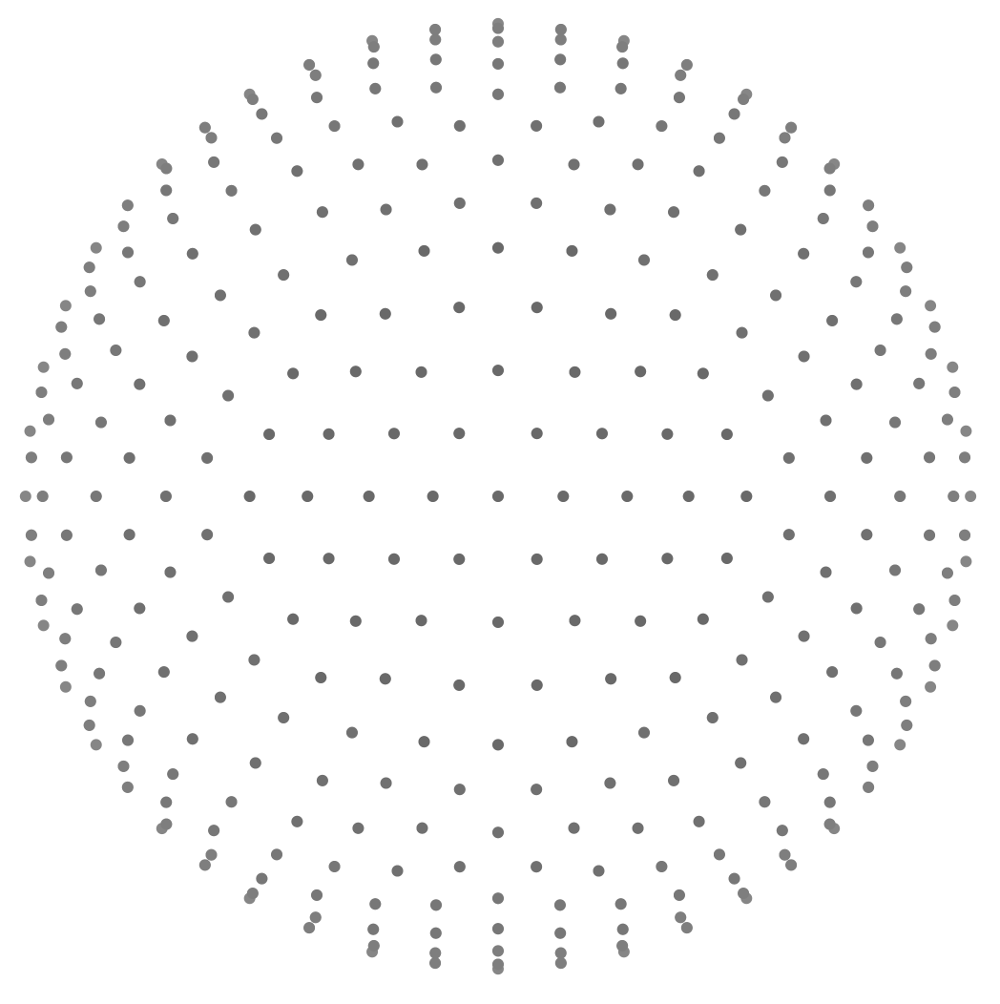
\includegraphics[height=2in]{figures/geodesicGrid3}
		\caption{3 subdivisions}
	\end{subfigure}
	\begin{subfigure}{0.49\textwidth}
		\centering
		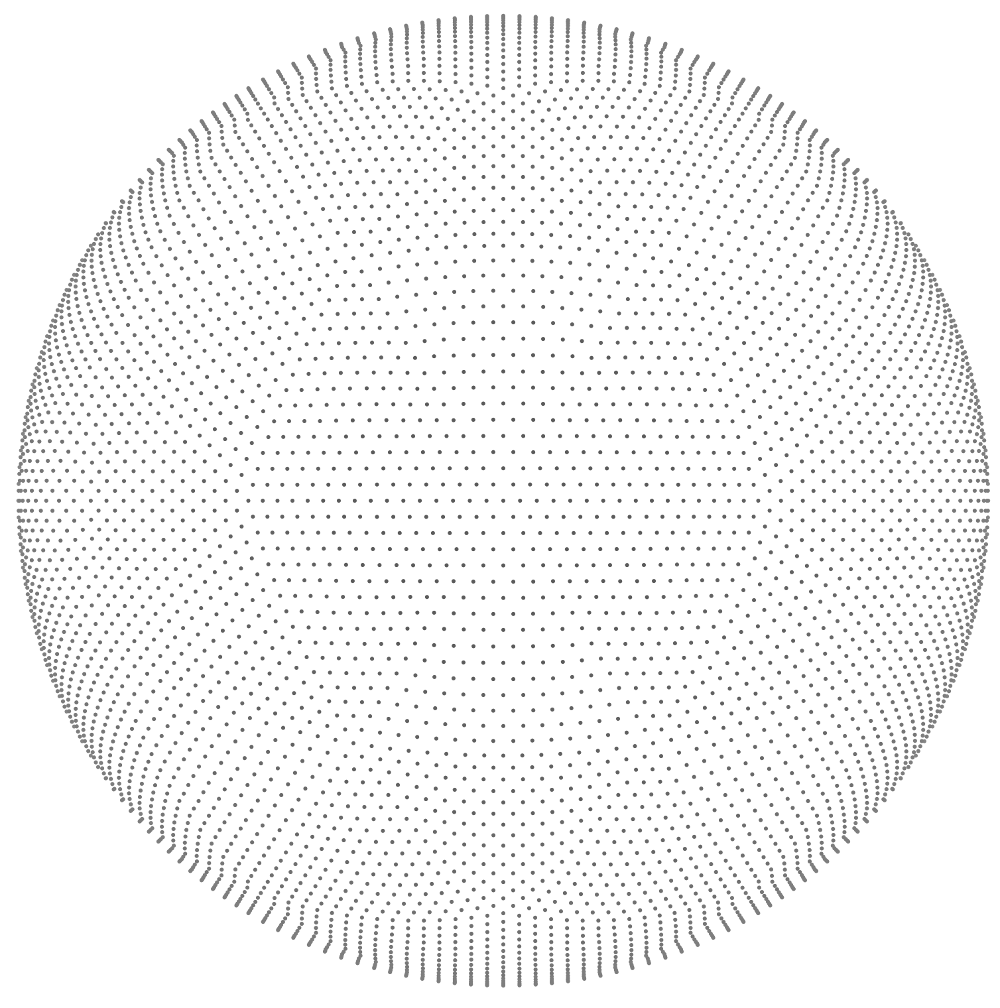
\includegraphics[height=2in]{figures/geodesicGrid5}
		\caption{5 subdivisions}
	\end{subfigure}
	\caption{
		Fast near-uniform sampling of the sphere using icosahedral approximations.
	}
	\label{fig:geodesicGrid}
\end{figure}

For more advanced linear algebra (often used in the analysis of RDC data), {\libprotnmr} integrates with the Jama library to perform these computations, including principal component analysis, eigenvalue/spectral decomposition, singular value decomposition, and QR factorization. Numerical error resulting from the usage of {\libprotnmr}'s geometry and mathematical libraries is handled in a rudimentary way by using epsilon-based comparison of floating point numbers. However, when exact precision is actually needed, critical methods can be implemented using multi-precision floating point numbers, or exact number types using the computational geometry algorithms library (CGAL).


\section{Visualization using KiNG}

When working with geometric data, visualizing the results of computations in three-dimensions (even intermediate computations) can often provide much more insight than tables, plots, and debuggers. For this reason, many of the geometrical objects provided by {\libprotnmr} can be rendered into a Kinemage for use with the 3D display software KiNG. \figreftwo{fig:kingProtein}{fig:kingAdvanced} show examples of the kinds of geometry that can be rendered with {\libprotnmr} and KiNG. Example code for creating Kinemages is presented in \coderef{code:king}.

\begin{codesample}
	\caption{
		Display 3D geometry using KiNG.
	}
	\begin{minted}[gobble=2,mathescape]{java}
		// render the sphere samples from $\figref{fig:geodesicGrid}$
		GeodesicGrid grid = new GeodesicGrid( 5 );
		Kinemage kin = new Kinemage();
		KinemageBuilder.appendPoints( kin, grid.vertices() );
		new KinemageWriter().show( kin );
		
		// show a protein structure, and wait for the user
		Protein protein = getProteinFromSomewhere();
		kin = new Kinemage();
		KinemageBuilder.appendAxes( kin );
		KinemageBuilder.appendProtein( kin, protein );
		new KinemageWriter().showAndWait( kin );
	\end{minted}
	\label{code:king}
\end{codesample}

\begin{figure}
	\centering
	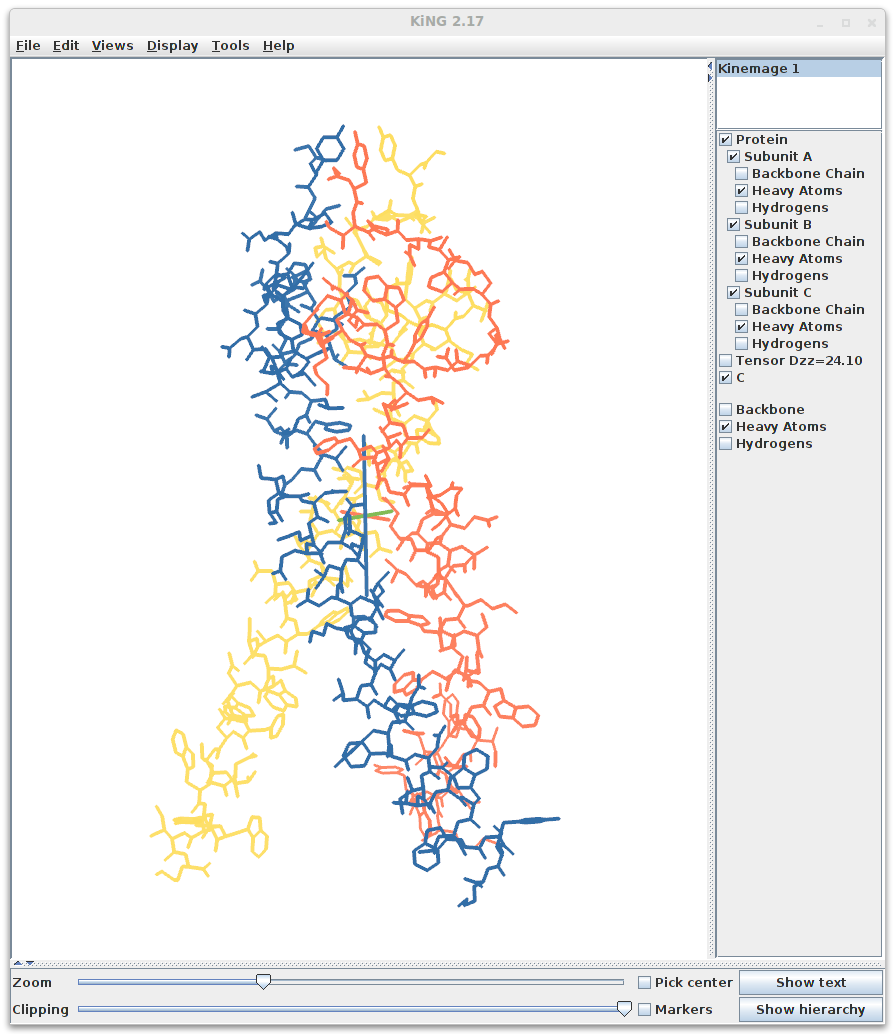
\includegraphics[height=4in]{figures/kingProtein}
	\caption{
		a protein structure rendered by {\libprotnmr} in KiNG along with the principal axes of the alignment.
	}
	\label{fig:kingProtein}
\end{figure}

\begin{figure}
	\centering
	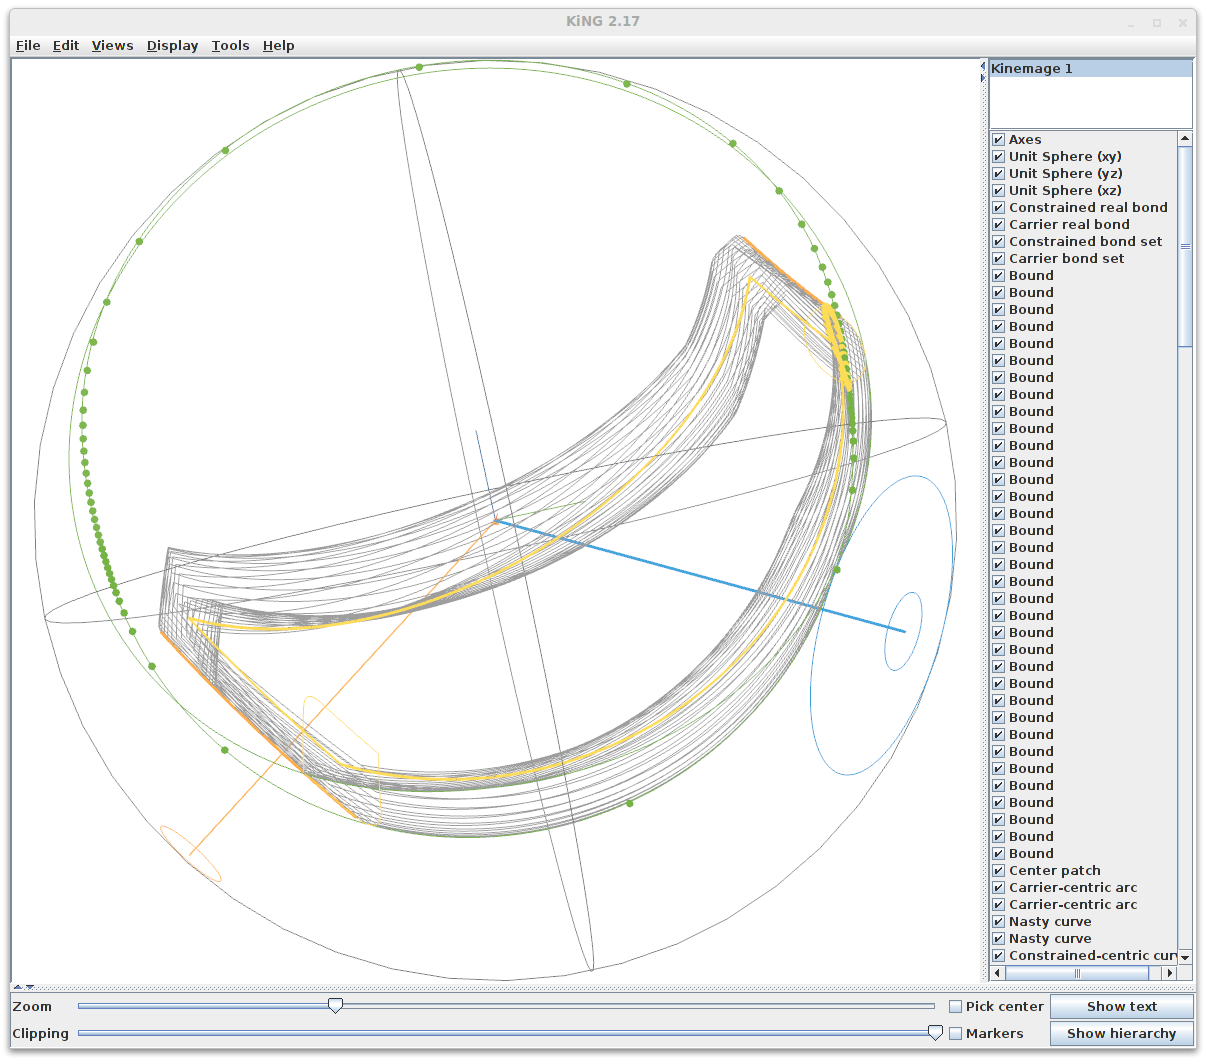
\includegraphics[height=4in]{figures/kingAdvanced}
	\caption{
		Viewing complicated abstract geometry is also possible using KiNG.
	}
	\label{fig:kingAdvanced}
\end{figure}


\section{Plotting}

While KiNG is great for interacting with 3D graphics, it is not terribly great for rendering publication-quality figures. For this, {\libprotnmr} provides a plotting module that builds on the popular open source \software{JFreeChart} library. Plotting is limited to 2D displays of information, so it cannot render protein structures, but \software{PyMol} is the typical choice for that task anyway. {\libprotnmr}'s plotting module can plot various specialized graphs though, including comparisons of experimental vs back-computed RDC values (\coderef{code:plots}), RDC histograms, representations of functions over the sphere (\figref{fig:plotSphere}), geometry in the plane (\figref{fig:dagkMsrs}), even geometry in phi,psi space like Ramachandran statistics.

\begin{codesample}
	\caption{
		Rendering specialized plots takes only a few lines of code.
	}
	\begin{minted}[gobble=2]{java}
		Protein protein = getProtein();
		List<Rdc<AtomAddressInternal>> rdcs = getRdcs();
		AlignmentTensor tensor = AlignmentTensor.compute(
			protein, rdcs
		);
		ChartWriter.showAndWait(
			Plotter.plotRdcFit( rdcs, tensor, protein )
		);
	\end{minted}
	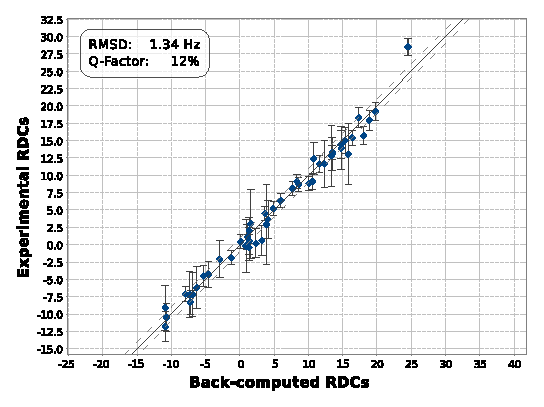
\includegraphics[width=4in]{figures/rdcFit2M7W}
	\label{code:plots}
\end{codesample}

\begin{figure}
	\centering
	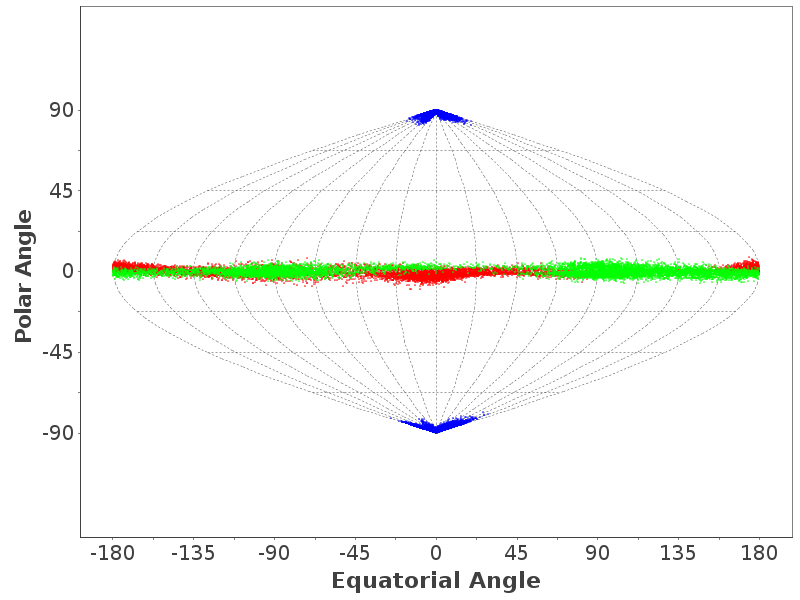
\includegraphics[width=4in]{figures/plotSphere}
	\caption[Plotting functions defined over the sphere]{
		{\libprotnmr} can plot functions over the sphere using a Sanson-Flamsteed projection.
	}
	\label{fig:plotSphere}
\end{figure}


\section{Utilities}

{\libprotnmr} has a number of utility classes that perform tasks not necessarily related to structural biology, but nonetheless are useful tools for building software that performs structural biological computations. There are many tools that fall into this category, but three of them are widely used and applicable to many situations: the timer, the profiler, and the progress bar. Since structural biological algorithms often perform very sophisticated computations, these computations can take a lot of wall clock time. These three tools are designed to help manage software performance and also the time of the computational scientist. The timer does just what you think it should. It measures wall clock time between defined start and end lines of code (See \coderef{code:timer}). The profiler is also very straightforward. Of course, many full-featured tools for profiling software exist, but sometimes the simple tools are the most useful. The profiler in {\libprotnmr} works in much the same way the timer does. Start and end lines of code are defined, and the wall clock time between them is measured. Where it differs from the timer though, is that each period of time is collected into user-defined bins and the final aggregate running times can be reported (See \coderef{code:profiler}). This allows the computational scientist to quickly narrow down on performance bottlenecks in the software just by writing a few lines of code without having to rely on complicated or cumbersome profiling frameworks.

\begin{codesample}
	\caption{
		Timers provide a simple way to report the running time of algorithms.
	}
	\begin{minted}[gobble=2]{java}
		Timer timer = new Timer();
		timer.start();
		doSomethingComplicated();
		System.out.println( timer.getElapsedTime() );
	\end{minted}
	\label{code:timer}
\end{codesample}

\begin{codesample}
	\caption{
		Profilers are a useful and simple tool to find performance bottlenecks.
	}
	\begin{minted}[gobble=2]{java}
		Profiler.start( "total" );
		while( condition )
		{
			doSomethingUnimportant();
			Profiler.start( "important" );
			doSomethingImportant();
			Profiler.stop( "important" );
			doSomethingUnimportant();
		}
		Profiler.stop( "total" );
		System.out.println( Profiler.getReport() );
		System.out.println( Profiler.getMemoryUsed() );
	\end{minted}
	\label{code:profiler}
\end{codesample}

Perhaps the most useful of the three tools is the progress bar (\coderef{code:progressBar}). The progress bar is initialized with a number of units of work to be performed. Then during execution of the software, the progress bar is updated with the number of units of work completed. Not only can the progress bar then periodically report what percentage of the work has been completed, but it also attempts to estimate the amount of wall clock time remaining until the end of the task. Since both linear and quadratic prediction models are available to the progress bar, it can fairly accurately predict the time remaining for a wide range of tasks. This tool lets the computational scientist decide shortly after the start of a long computation whether or not it would be worth the time to wait for the results.

\begin{codesample}
	\caption{
		Progress bars show long one might have to wait for a result.
	}
	\begin{minted}[gobble=2]{java}
		Progress progress = new Progress( 1000, 5000 );
		for( int i=0; i<1000; i++ )
		{
			doWork();
			progress.incrementProgress();
			// running time estimates are automatically
			// written to stdout every 5000 ms
			// a final report is written at 100%
		}
		
		// if an algorithm has quadratic running time,
		// a different prediction model can be used
		progress = new Progress( 1000, 5000, Model.Quadratic );
		for( int i=0; i<1000; i++ )
		{
			doQuadraticWork( i );
			progress.incrementProgress();
		}
	\end{minted}
	\label{code:progressBar}
\end{codesample}


\section{Python bindings}

All of the functionality in {\libprotnmr} is accessible to Python scripts as well as Java applications thanks to the JPype compatibility layer. The flexibility of a scripting environment allows many separate or short tasks to be completed using {\libprotnmr} when writing a full-blown Java application would be overkill (\coderef{code:python}).

\begin{codesample}
	\caption{
		Python bindings make {\libprotnmr}'s catalog of modules available in a scripting environment.
	}
	\begin{minted}[gobble=2]{python}
		import jvm, libprotnmr
		
		# start the jvm
		jvmInstance = jvm.Jvm()
		jvmInstance.addPath( "libprotnmr.jar" )
		libprotnmr.initJvm( jvmInstance )
		jvmInstance.start( "-Xmx512m" )
		
		# call libprotnmr functions for common tasks
		protein = libprotnmr.loadProtein( "path/to/protein.pdb" )
		rdcs = libprotnmr.loadRdcs( "path/to/rdcs.mr" )
		rdcs = libprotnmr.mapRdcsToProtein( rdcs, protein )

		# import Java class names to use other modules directly
		AlignmentTensor = libprotnmr.f.nmr.AlignmentTensor
		
		# compute an RDC fit
		tensor = AlignmentTensor.compute( protein, rdcs )
		print "RDC Q-factor: %.1f"
			% tensor.getQFactor( protein, rdcs )*100
	\end{minted}
	\label{code:python}
\end{codesample}

\end{document}
